\documentclass[12pt,a4paper]{article}
\usepackage[utf8]{vietnam}
\usepackage{amsmath,amssymb}
\usepackage{tabularx}
\usepackage{tikz}
\usetikzlibrary{calc,angles,quotes,arrows.meta,patterns}
\usepackage{xcolor}
\usepackage{enumitem}
\usepackage{fancyhdr}
\usepackage{graphicx}
\usepackage[top=0.9cm, bottom=0.9cm, left=1.2cm, right=1.2cm]{geometry}
\usepackage[sol]{ex_test}
\SAOPTN{widthSA=3.2,heightSA=0.62}

\setlength{\headheight}{15pt}
\setlength{\parskip}{0pt}

\pagestyle{fancy}
\fancyhf{}
\rhead{\textit{Hướng dẫn giải chi tiết -- Đề số 09}}
\lhead{\textit{Môn Toán 9 -- Giữa học kì I}}
\cfoot{\thepage}

\begin{document}

\begin{center}
  \textbf{\Large HƯỚNG DẪN GIẢI CHI TIẾT -- ĐỀ SỐ 09}\\
  \textbf{\large MÔN TOÁN 9 -- GIỮA HỌC KỲ I}
\end{center}
\vspace{2mm}

% --- BẢNG ĐÁP ÁN TỔNG HỢP ---
\noindent\textbf{\large I. BẢNG ĐÁP ÁN TỔNG HỢP}

\vspace{1mm}
\noindent\textbf{1. Phần I - Trắc nghiệm nhiều phương án lựa chọn (3,0 điểm):}
\begin{center}
\begin{tabular}{|c|c|c|c|c|c|c|c|c|c|c|c|c|}
\hline
\textbf{Câu} & \textbf{1} & \textbf{2} & \textbf{3} & \textbf{4} & \textbf{5} & \textbf{6} & \textbf{7} & \textbf{8} & \textbf{9} & \textbf{10} & \textbf{11} & \textbf{12} \\
\hline
\textbf{Chọn} & \textbf{C} & \textbf{D} & \textbf{B} & \textbf{B} & \textbf{A} & \textbf{A} & \textbf{D} & \textbf{A} & \textbf{B} & \textbf{C} & \textbf{D} & \textbf{B} \\
\hline
\end{tabular}
\end{center}
\vspace{1mm}

\noindent\textbf{2. Phần II - Trắc nghiệm Đúng/Sai (2,0 điểm):}
\begin{center}
\begin{tabular}{|c|c|c|c|c||c|c|c|c|c|}
\hline
\textbf{Câu} & \textbf{Lệnh hỏi} & \textbf{Đúng} & \textbf{Sai} & \textbf{Điểm} & \textbf{Câu} & \textbf{Lệnh hỏi} & \textbf{Đúng} & \textbf{Sai} & \textbf{Điểm} \\
\hline
 & a) & \textbf{X} & & 0,1 & & a) & \textbf{X} & & 0,1 \\
\cline{2-5}\cline{7-10}
\textbf{1} & b) & \textbf{X} & & 0,25 & \textbf{2} & b) & \textbf{X} & & 0,25 \\
\cline{2-5}\cline{7-10}
 & c) & \textbf{X} & & 0,5 & & c) & \textbf{X} & & 0,5 \\
\cline{2-5}\cline{7-10}
 & d) & \textbf{X} & & 1,0 & & d) & \textbf{X} & & 1,0 \\
\hline
\end{tabular}
\end{center}
\vspace{1mm}

\noindent\textbf{3. Phần III - Trả lời ngắn (1,0 điểm):}
\begin{center}
\begin{tabular}{|c|c|c|}
\hline
\textbf{Câu} & \textbf{1} & \textbf{2} \\
\hline
\textbf{Đáp án} & $\mathbf{(2; 1)}$ & $\mathbf{4{,}8\text{ cm}}$ \\
\hline
\end{tabular}
\end{center}
\vspace{3mm}

% --- LỜI GIẢI CHI TIẾT ---
\noindent\textbf{\large II. HƯỚNG DẪN GIẢI CHI TIẾT}

\vspace{2mm}
\noindent\textbf{\large PHẦN I. CÂU TRẮC NGHIỆM NHIỀU PHƯƠNG ÁN LỰA CHỌN}
\vspace{1mm}
\begin{ex}
Phương trình nào sau đây là phương trình bậc nhất hai ẩn?
\choice
{$2x - 4 = 0$}
{$5y - 1 = 3(y - 4)$}
{\True $2x + 7y = 5$}
{$2x^2 + 8y = 0$}
\loigiai{
Phương trình bậc nhất hai ẩn có dạng $ax + by = c$, trong đó các hệ số $a, b$ không đồng thời bằng 0 và các ẩn $x, y$ đều có bậc 1. Do đó $2x + 7y = 5$ là phương trình bậc nhất hai ẩn.
}
\end{ex}

\begin{ex}
Cặp số $(2; 0)$ là nghiệm của hệ phương trình nào sau đây?
\choice
{$\begin{cases} 2x - 2y = 2 \\ x + 2y = 4 \end{cases}$}
{$\begin{cases} 2x - y = -1 \\ 3x - y = 8 \end{cases}$}
{$\begin{cases} 2x - y = -1 \\ 3x - y = 7 \end{cases}$}
{\True $\begin{cases} 4x - 2y = 8 \\ 3x - 5y = 6 \end{cases}$}
\loigiai{
Thay $(x; y) = (2; 0)$ vào hệ ở phương án D: $4(2) - 2(0) = 8$ (đúng) và $3(2) - 5(0) = 6$ (đúng). Do đó $(2; 0)$ là nghiệm của hệ phương trình này.
}
\end{ex}

\begin{ex}
Hệ phương trình nào sau đây là hệ hai phương trình bậc nhất hai ẩn?
\choice
{$\begin{cases} 2x - y = 3 \\ 2x^2 + 3y = 4 \end{cases}$}
{\True $\begin{cases} 3x - y = -1 \\ 5x - 3y = 8 \end{cases}$}
{$\begin{cases} 3x - 2y = 1 \\ \frac{1}{x} - 3y = 7 \end{cases}$}
{$\begin{cases} 2x - y^2 = 4 \\ 2x - 3y = 5 \end{cases}$}
\loigiai{
Hệ hai phương trình bậc nhất hai ẩn gồm hai phương trình mà mỗi phương trình đều là bậc nhất hai ẩn $x, y$. Phương án B thỏa mãn.
}
\end{ex}

\begin{ex}
Khẳng định nào sau đây là đúng với mọi $A \ge 0, B \ge 0$?
\choice
{$\sqrt{A \cdot B} = \sqrt{A} \cdot \sqrt{B}$ ($A \ge 0, B > 0$)}
{\True $\sqrt{A \cdot B} = \sqrt{A} \cdot \sqrt{B}$ ($A \ge 0, B \ge 0$)}
{$\sqrt{A \cdot B} = \sqrt{A} \cdot \sqrt{B}$ ($AB \ge 0$)}
{$\sqrt{A \cdot B} = \sqrt{A} \cdot \sqrt{B}$ ($A > 0, B > 0$)}
\loigiai{
Với hai biểu thức không âm $A \ge 0, B \ge 0$, ta có quy tắc khai phương một tích: $\sqrt{A \cdot B} = \sqrt{A} \cdot \sqrt{B}$.
}
\end{ex}

\begin{ex}
Với $a < 3$, kết quả rút gọn của biểu thức $\sqrt{(a - 3)^2} - 2(a + 1)$ là:
\choice
{\True $1 - 3a$}
{$-a - 1$}
{$-a - 5$}
{$5 - 3a$}
\loigiai{
Ta có $\sqrt{(a - 3)^2} = |a - 3|$. Vì $a < 3$ nên $a - 3 < 0 \implies |a - 3| = 3 - a$. Khi đó biểu thức bằng: $(3 - a) - 2(a + 1) = 3 - a - 2a - 2 = 1 - 3a$.
}
\end{ex}

\begin{ex}
Kết quả của phép tính $\sqrt{\frac{49}{169} \cdot 0{,}36}$ là:
\choice
{\True $\frac{21}{65}$}
{$\frac{35}{33}$}
{$\frac{42}{13}$}
{$\frac{42}{169}$}
\loigiai{
Áp dụng quy tắc nhân và khai căn: $\sqrt{\frac{49}{169} \cdot 0{,}36} = \sqrt{\frac{49}{169}} \cdot \sqrt{0{,}36} = \frac{7}{13} \cdot 0{,}6 = \frac{7}{13} \cdot \frac{3}{5} = \frac{21}{65}$.
}
\end{ex}

\newpage
\begin{ex}
Cho $a > b$, kết luận nào sau đây không đúng?
\choice
{$-a < -b$}
{$-2a < -2b$}
{$a - b > 0$}
{\True $a^2 > b^2$}
\loigiai{
Khi nhân hoặc chia với số âm, bất đẳng thức đổi chiều (A và B đúng). Hiệu $a - b > 0$ là định nghĩa của $a > b$ (C đúng). Khẳng định D không đúng trong trường hợp số âm, ví dụ: $1 > -3$ nhưng $1^2 = 1 < (-3)^2 = 9$.
}
\end{ex}

\begin{ex}
Cho tam giác $MNP$ vuông tại $M$ có đường cao $MH$ và góc $\widehat{N} = \alpha$. Tỉ số lượng giác $\cos \alpha$ bằng:
\choice
{\True $\frac{NH}{MN}$}
{$\frac{MP}{MH}$}
{$\frac{MP}{MN}$}
{$\frac{MH}{NM}$}
\loigiai{
Xét tam giác vuông $MNH$ vuông tại $H$, góc nhọn $\widehat{N} = \alpha$. Theo định nghĩa, $\cos \alpha = \frac{\text{cạnh kề}}{\text{cạnh huyền}} = \frac{NH}{MN}$.
}
\end{ex}

\begin{ex}
Trong hình vẽ, bạn Minh đứng ở vị trí $M$, bạn Nam đứng ở vị trí $N$ cùng ở một bên lề đường và cây xanh $C$ nằm đối diện vị trí Nam đứng ở phía bên kia đường. Biết $MN = 3{,}9\text{ m}$ và góc $\widehat{NMC} = 72^\circ$. Tính khoảng cách từ Minh đến cây xanh $C$ (làm tròn kết quả đến hàng đơn vị):
\begin{center}
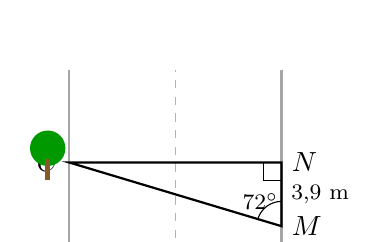
\begin{tikzpicture}[scale=0.9]
  \draw[thick, gray!70] (-1.5,-1.3) -- (-1.5,1.3);
  \draw[thick, gray!70] (1.5,-1.3) -- (1.5,1.3);
  \draw[dashed, gray!60] (0,-1.3) -- (0,1.3);
  \coordinate (C) at (-1.5,0);
  \coordinate (N) at (1.5,0);
  \coordinate (M) at (1.5,-0.9);
  \draw[thick] (C) node[left]{$C$} -- (N) node[right]{$N$} -- (M) node[right]{$M$} -- cycle;
  \draw (N) ++(-0.25,0) -- ++(0,-0.25) -- ++(0.25,0);
  \draw (M) ++(0,0.35) arc (90:162:0.35);
  \node at (1.2,-0.55) {\footnotesize $72^\circ$};
  \node[right] at (1.5,-0.45) {\footnotesize $3{,}9\text{ m}$};
  \fill[green!60!black] (-1.8,0.2) circle (0.25);
  \draw[line width=1.8pt, brown!70!black] (-1.8,0.05) -- (-1.8,-0.25);
\end{tikzpicture}
\end{center}
\choice
{$12\text{ m}$}
{\True $13\text{ m}$}
{$12{,}7\text{ m}$}
{$12{,}6\text{ m}$}
\loigiai{
Tam giác $MNC$ vuông tại $N$. Áp dụng tỉ số lượng giác của góc nhọn $\widehat{M} = 72^\circ$:\par $\cos M = \frac{MN}{MC} \implies MC = \frac{MN}{\cos 72^\circ} = \frac{3{,}9}{\cos 72^\circ} \approx \frac{3{,}9}{0{,}3090} \approx 12{,}62\text{ m}$.\par Làm tròn đến hàng đơn vị là $13\text{ m}$.
}
\end{ex}

\begin{ex}
Cho $a > b$, khi đó ta có khẳng định nào đúng?
\choice
{$2a < 2b$}
{$-2a > -2b$}
{\True $2a - 3 > 2b - 3$}
{$-3a - 5 > -3b - 5$}
\loigiai{
Vì $a > b \implies 2a > 2b \implies 2a - 3 > 2b - 3$. Khẳng định C đúng.
}
\end{ex}

\begin{ex}
Cho bất đẳng thức $2a + b \ge 3a$. Vế trái của bất đẳng thức là:
\choice
{$3a$}
{$b$}
{$2a$}
{\True $2a + b$}
\loigiai{
Vế trái của bất đẳng thức $2a + b \ge 3a$ là biểu thức nằm ở bên trái dấu so sánh, tức là $2a + b$.
}
\end{ex}

\begin{ex}
Cho tam giác $ABC$ vuông tại $A$. Tỉ số $\sin B$ bằng:
\choice
{$\frac{AB}{BC}$}
{\True $\frac{AC}{BC}$}
{$\frac{AB}{AC}$}
{$\frac{AC}{AB}$}
\loigiai{
Trong tam giác $ABC$ vuông tại $A$, cạnh đối của góc $B$ là $AC$ và cạnh huyền là $BC$. Do đó $\sin B = \frac{AC}{BC}$.
}
\end{ex}


\newpage
\noindent\textbf{\large PHẦN II. CÂU TRẮC NGHIỆM ĐÚNG SAI}
\vspace{1mm}
\begin{ex}
Cho hệ phương trình $\begin{cases} 2x + y = 4 \\ x - y = 2. \end{cases}$ Xét tính Đúng/Sai của các khẳng định sau:
\choiceTF
{\True Cặp số $(2; 0)$ là nghiệm của phương trình thứ nhất.}
{\True Cộng từng vế hai phương trình của hệ ta được phương trình $3x = 6$.}
{\True Nghiệm của hệ phương trình là $(2; 0)$.}
{\True Giá trị biểu thức $M = x^2 - y^2$ tại nghiệm của hệ bằng $4$.}
\loigiai{
\begin{itemize}[leftmargin=*]
  \item a) Đúng. Thay $x = 2, y = 0$ vào phương trình $2x + y = 4$: $2(2) + 0 = 4$ (đúng). Khẳng định Đúng.
  \item b) Đúng. Cộng vế theo vế: $(2x + y) + (x - y) = 4 + 2 \iff 3x = 6$. Khẳng định Đúng.
  \item c) Đúng. Từ $3x = 6 \implies x = 2$. Thay vào $x - y = 2 \implies 2 - y = 2 \implies y = 0$. Nghiệm là $(2; 0)$. Khẳng định Đúng.
  \item d) Đúng. Thay $(x; y) = (2; 0)$ vào $M$: $M = 2^2 - 0^2 = 4$. Khẳng định Đúng.
\end{itemize}
}
\end{ex}

\begin{ex}
Cho tam giác $ABC$ vuông tại $A$, đường cao $AH$. Biết $BH = 2\text{ cm}$ và $CH = 8\text{ cm}$. Xét tính Đúng/Sai của các khẳng định sau:
\choiceTF
{\True Độ dài đường cao $AH = 4\text{ cm}$.}
{\True Độ dài cạnh huyền $BC = 10\text{ cm}$.}
{\True Độ dài cạnh $AB = \sqrt{20}\text{ cm}$.}
{\True Giá trị của $\sin B = \frac{2}{\sqrt{5}}$.}
\loigiai{
\begin{itemize}[leftmargin=*]
  \item a) Đúng. Theo hệ thức lượng: $AH^2 = BH \cdot CH = 2 \cdot 8 = 16 \implies AH = 4\text{ cm}$. Khẳng định Đúng.
  \item b) Đúng. Ta có $BC = BH + CH = 2 + 8 = 10\text{ cm}$. Khẳng định Đúng.
  \item c) Đúng. Theo hệ thức lượng: $AB^2 = BH \cdot BC = 2 \cdot 10 = 20 \implies AB = \sqrt{20}\text{ cm} = 2\sqrt{5}\text{ cm}$. Khẳng định Đúng.
  \item d) Đúng. Xét tam giác vuông $ABH$ vuông tại $H$: $\sin B = \frac{AH}{AB} = \frac{4}{\sqrt{20}} = \frac{4}{2\sqrt{5}} = \frac{2}{\sqrt{5}}$. Khẳng định Đúng.
\end{itemize}
}
\end{ex}


\vspace{2mm}
\noindent\textbf{\large PHẦN III. CÂU TRẢ LỜI NGẮN}
\vspace{1mm}
\begin{ex}
Giải hệ phương trình $\begin{cases} 3x - 2y = 4 \\ x + 2y = 4. \end{cases}$ Tìm nghiệm $(x; y)$.
\shortans{$(2; 1)$}
\loigiai{
Cộng hai phương trình vế theo vế: $4x = 8 \implies x = 2$. Thay $x = 2$ vào phương trình thứ hai: $2 + 2y = 4 \implies 2y = 2 \implies y = 1$. Vậy nghiệm là $(2; 1)$.
}
\end{ex}

\begin{ex}
Cho tam giác $ABC$ vuông tại $A$, đường cao $AH$. Biết $AB = 6\text{ cm}$ và $AC = 8\text{ cm}$. Tính độ dài đường cao $AH$.
\shortans{$4{,}8\text{ cm}$}
\loigiai{
Áp dụng định lí Pythagore: $BC = \sqrt{AB^2 + AC^2} = \sqrt{6^2 + 8^2} = 10\text{ cm}$. Áp dụng hệ thức lượng: $AH \cdot BC = AB \cdot AC \implies AH = \frac{6 \cdot 8}{10} = 4{,}8\text{ cm}$.
}
\end{ex}


\newpage
\noindent\textbf{\large PHẦN IV. TỰ LUẬN}
\vspace{1mm}
\noindent\textbf{Câu 1 (1,5 điểm).}

Giải các hệ phương trình sau:\par a) $\begin{cases} x + 3y = 2 \\ x + 2y = 5 \end{cases}$\par b) $\begin{cases} 4x - 3y = -1 \\ 2x + 3y = 13. \end{cases}$

\noindent\textbf{Lời giải:}

a) Trừ phương trình thứ hai cho phương trình thứ nhất vế theo vế: $(x + 3y) - (x + 2y) = 2 - 5 \implies y = -3$.\par Thay $y = -3$ vào phương trình thứ nhất: $x + 3(-3) = 2 \iff x - 9 = 2 \implies x = 11$.\par Vậy hệ có nghiệm duy nhất là $(11; -3)$.\par b) Cộng hai phương trình vế theo vế: $(4x - 3y) + (2x + 3y) = -1 + 13 \iff 6x = 12 \implies x = 2$.\par Thay $x = 2$ vào phương trình thứ hai: $2(2) + 3y = 13 \iff 4 + 3y = 13 \iff 3y = 9 \implies y = 3$.\par Vậy hệ có nghiệm duy nhất là $(2; 3)$.

\vspace{3mm}
\noindent\textbf{Câu 2 (1,0 điểm).}

Trong kỳ thi tuyển sinh vào lớp 10 Trung học phổ thông, tổng số học sinh dự thi của hai trường THCS $A$ và $B$ là 180 em, tổng số học sinh trúng tuyển là 157 em. Tính số học sinh dự thi và số học sinh trúng tuyển của từng trường, biết trường $A$ có $90\%$ học sinh dự thi trúng tuyển và trường $B$ có $85\%$ học sinh dự thi trúng tuyển.

\noindent\textbf{Lời giải:}

Gọi số học sinh dự thi của trường $A$ và trường $B$ lần lượt là $x$ và $y$ ($x, y \in \mathbb{N}^*, x, y < 180$).\par Tổng số học sinh dự thi của hai trường là 180 em: $x + y = 180 \quad (1)$.\par Số học sinh trúng tuyển của trường $A$ là $90\% x = 0{,}9x$ và trường $B$ là $85\% y = 0{,}85y$.\par Tổng số học sinh trúng tuyển là 157 em: $0{,}9x + 0{,}85y = 157 \quad (2)$.\par Từ (1) và (2) ta có hệ phương trình: $\begin{cases} x + y = 180 \\ 0{,}9x + 0{,}85y = 157 \end{cases}$\par Nhân hai vế phương trình đầu với 0,9: $\begin{cases} 0{,}9x + 0{,}9y = 162 \\ 0{,}9x + 0{,}85y = 157 \end{cases}$\par Trừ vế theo vế: $0{,}05y = 5 \implies y = 100$ (thỏa mãn).\par Suy ra $x = 180 - 100 = 80$ (thỏa mãn).\par Số học sinh trúng tuyển trường $A$: $80 \cdot 90\% = 72$ học sinh.\par Số học sinh trúng tuyển trường $B$: $100 \cdot 85\% = 85$ học sinh.\par Vậy trường $A$ có 80 em dự thi (72 em trúng tuyển), trường $B$ có 100 em dự thi (85 em trúng tuyển).

\vspace{3mm}
\newpage
\noindent\textbf{Câu 3 (1,0 điểm).}

a) Cho tam giác $DEF$ vuông tại $D$ có $DE = 9\text{ cm}, \widehat{F} = 35^\circ$. Hãy giải tam giác vuông $DEF$ (độ dài các cạnh làm tròn đến hàng phần trăm).\par b) Hai chiếc thuyền $A$ và $B$ ở vị trí được minh họa như hình vẽ. Tính khoảng cách giữa chúng (làm tròn đến hàng phần mười của mét). Biết độ dài $IK = 500\text{ m}, \widehat{AKI} = 50^\circ, \widehat{AKB} = 15^\circ$.
\begin{center}
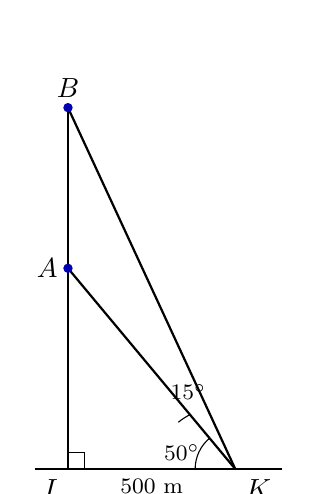
\begin{tikzpicture}[scale=0.85]
  \coordinate (I) at (0,0);
  \coordinate (K) at (2.5,0);
  \coordinate (A) at (0,3.0);
  \coordinate (B) at (0,5.4);
  \draw[thick] (-0.5,0) -- (3.2,0);
  \draw[thick] (I) node[below left]{$I$} -- (K) node[below right]{$K$};
  \draw[thick] (I) -- (B) node[above]{$B$};
  \draw[thick] (K) -- (A) node[left]{$A$};
  \draw[thick] (K) -- (B);
  \draw (I) ++(0,0.25) -- ++(0.25,0) -- ++(0,-0.25);
  \draw (K) ++(-0.6,0) arc (180:130:0.6);
  \node at (1.7,0.25) {\footnotesize $50^\circ$};
  \draw (K) ++(-0.85,0.7) arc (130:115:0.85);
  \node at (1.8,1.15) {\footnotesize $15^\circ$};
  \node[below] at (1.25,0) {\footnotesize $500\text{ m}$};
  \fill[blue!70!black] (A) circle (2pt);
  \fill[blue!70!black] (B) circle (2pt);
\end{tikzpicture}
\end{center}

\noindent\textbf{Lời giải:}

a) Xét tam giác $DEF$ vuông tại $D$:\par - $\widehat{E} = 90^\circ - \widehat{F} = 90^\circ - 35^\circ = 55^\circ$.\par - $DF = DE \cdot \tan E = 9 \cdot \tan 55^\circ \approx 9 \cdot 1{,}4281 \approx 12{,}85\text{ cm}$.\par - $EF = \frac{DE}{\sin F} = \frac{9}{\sin 35^\circ} \approx \frac{9}{0{,}5736} \approx 15{,}69\text{ cm}$.\par b) Xét tam giác $AIK$ vuông tại $I$ có $\widehat{AKI} = 50^\circ$:\par $AI = IK \cdot \tan \widehat{AKI} = 500 \cdot \tan 50^\circ \approx 500 \cdot 1{,}1918 \approx 595{,}88\text{ m}$.\par Xét tam giác $BIK$ vuông tại $I$ có $\widehat{BKI} = \widehat{AKI} + \widehat{AKB} = 50^\circ + 15^\circ = 65^\circ$:\par $BI = IK \cdot \tan \widehat{BKI} = 500 \cdot \tan 65^\circ \approx 500 \cdot 2{,}1445 \approx 1072{,}25\text{ m}$.\par Khoảng cách giữa hai chiếc thuyền là đoạn $AB$:\par $AB = BI - AI \approx 1072{,}25 - 595{,}88 = 476{,}37\text{ m} \approx 476{,}4\text{ m}$.\par Vậy khoảng cách giữa hai thuyền là khoảng $476{,}4\text{ m}$.

\vspace{3mm}
\noindent\textbf{Câu 4 (0,5 điểm).}

Cho các số thực $x, y$ thỏa mãn $x^2 + y^2 - 4x + 2y + 5 = 0$. Tính giá trị của biểu thức $P = (x - 3)^{2026} + (y + 2)^{2026}$.

\noindent\textbf{Lời giải:}

Biến đổi phương trình giả thiết về tổng các bình phương:\par $(x^2 - 4x + 4) + (y^2 + 2y + 1) = 0 \iff (x - 2)^2 + (y + 1)^2 = 0$.\par Vì $(x - 2)^2 \ge 0$ và $(y + 1)^2 \ge 0$ với mọi $x, y \in \mathbb{R}$, nên đẳng thức xảy ra khi và chỉ khi:\par $\begin{cases} x - 2 = 0 \\ y + 1 = 0 \end{cases} \iff \begin{cases} x = 2 \\ y = -1. \end{cases}$\par Thay $x = 2$ và $y = -1$ vào biểu thức $P$ ta được:\par $P = (2 - 3)^{2026} + (-1 + 2)^{2026} = (-1)^{2026} + 1^{2026} = 1 + 1 = 2$.\par Vậy $P = 2$.

\vspace{3mm}

\vfill
\begin{center}
  \textbf{--- HẾT ---}
\end{center}
\end{document}
